\chapter{Επιμέρους συστήματα Κωδικοποιητή και Αποκωδικοποιητή}

\section{Σύστημα Υποδειγματοληψίας}

\par Το πρώτο κομμάτι της κωδικοποίησης είναι η υποδειγματοληψία του αρχικού σήματος. 
Έστω ότι το σήμα που μας δίνετε έχει προκύψει από δειγματοληψία ενός αναλογικού 
σήματος με συχνότητα δειγματοληψίας $f_{s1}$. Αρχικός στόχος του κωδικοποιητή 
είναι η μείωση της συχνότητας δειγματοληψίας στη $f_{s2}$, ώστε να μειωθούν τα δείγματα τα 
οποία χρησιμοποιούμε για να αναπαραστήσουμε το σήμα. Στην περίπτωση της αποκωδικοποίησης 
γίνεται υπερδειγματοληψία ώστε αυτό που θα προκύψει να έχει το ίδιο πλήθος δειγμάτων 
με το αρχικό σήμα. Κάνοντας αλλαγή στη συχνότητα δειγματοληψίας από την $f_{s1}$ στην 
$f_{s2}$ το νέο σήμα που προκύπτει έχει μήκος $floor(\frac{f_{s2}}{f_{s1}}\times
(length(x)-1))$.

\par Η συνάρτηση που υλοποιεί αυτή την διαδικασία είναι η 
\begin{lstlisting}[style=MyMatlab]
 function y=changefs(x,f_{s1},f_{s2},interpMethod)
\end{lstlisting}
όπου $f_{s1}$ η αρχική συχνότητα δειγματοληψίας και $f_{s2}$ η τελική και interpMethod είναι η μέθοδος 
με την οποία προκύπτουν τα δείγματα του y με τη μέθοδο της παρεμβολής. Το τέταρτο αυτό 
όρισμα δεν ζητείται από την εκφώνηση αλλά χρησιμοποιείται σε παρακάτω ερωτήματα. 
Στη συνάρτηση changefs ορίζουμε δύο μεταβλητές. Η πρώτη αντιστοιχεί στα δείγματα του αρχικού σήματος 
x, δηλαδή οριζεται ως πίνακας που έχει στοιχεία μέσα από το 1 έως το μήκος του x, 
ενώ η δεύτερη αντιπροσωπεύει τα δείγματα του y και δημιουργείται από το 1 έως το μήκος 
του x με βήμα $\frac{f_{s1}}{f_{s2}}$, έως το μήκος του x. Τα δύο αυτά διανύσματα 
δίνονται σαν είσοδο στην interp1 του Matlab και μας παράγουν το τελικό y, από το οποίο 
κρατάμε μόνο τα $floor(\frac{f_{s2}}{f_{s1}}\times(length(x)-1))$ πρώτα στοιχεία.

\noindent
\begin{minipage}{\linewidth}
\par Στη συνέχεια για να ελένξουμε την ορθότητα της υλοποίησης μας τρέχουμε την 
συνάρτηση testQ1. Παρακάτω παρουσιάζονται τα διαγράμματα που προκύπτουν.
\begin{figure}[H]
    \centering
\begin{subfigure}[h]{0.49\textwidth}
  \centering
  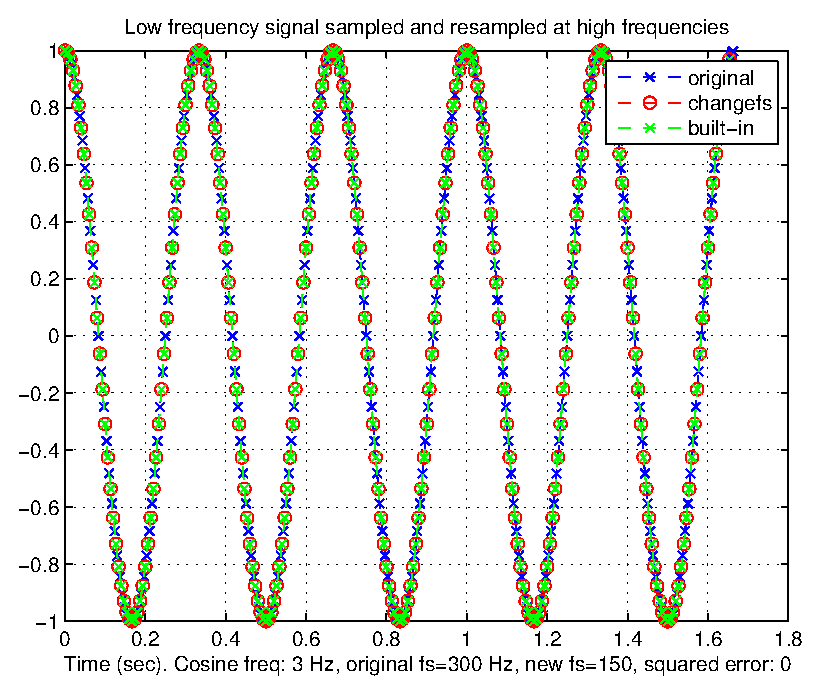
\includegraphics[width=0.35\paperwidth]{test11.eps}
  \caption{\protect{Δειγματοληψία σε συχνότητα μεγαλύτερης της Nyquist}}
\end{subfigure}
%~ \hfill
\begin{subfigure}[h]{0.49\textwidth}\centering
  \centering
  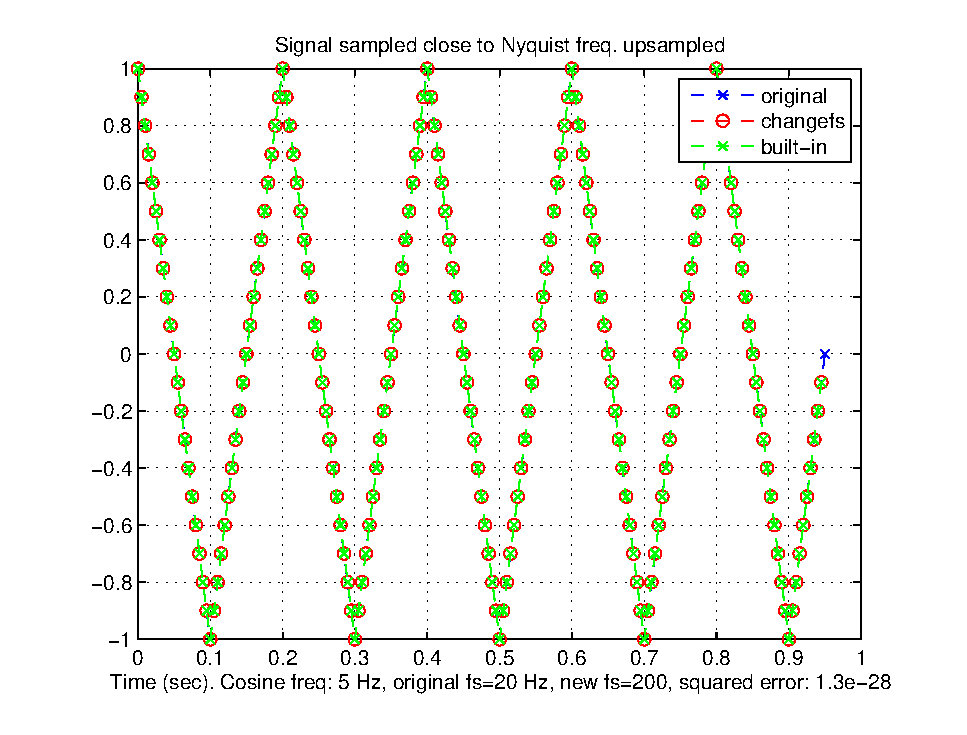
\includegraphics[width=0.35\paperwidth]{test12.eps}
  \caption{\protect{Δειγματοληψία σε συχνότητα κοντά στη Nyquist}}
  \end{subfigure}
  %~ \hfill
\begin{subfigure}[h]{0.49\textwidth}
  \centering
  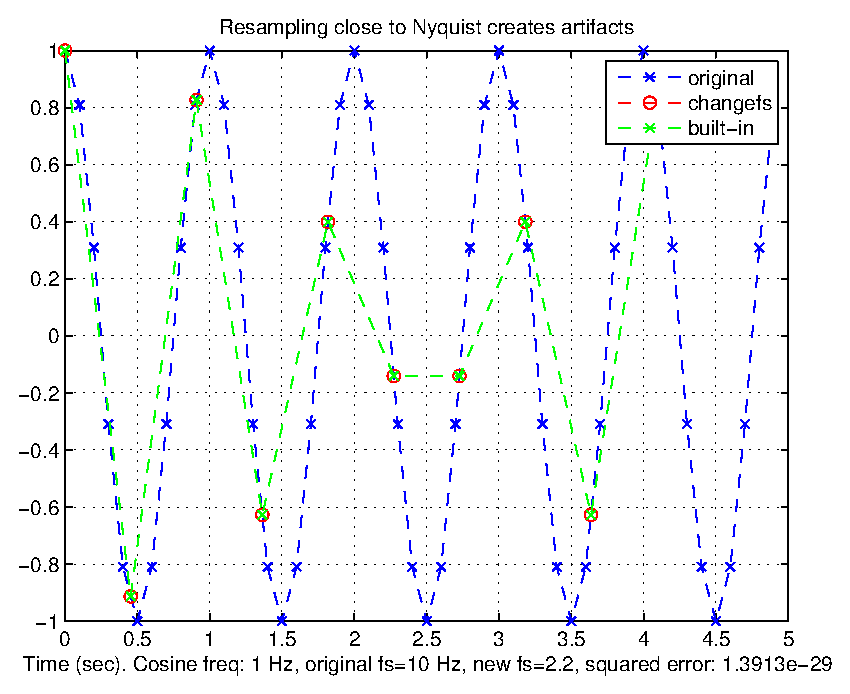
\includegraphics[width=0.35\paperwidth]{test13.eps}
  \caption{\protect{Δειγματοληψία σε συχνότητα πολύ κοντά στη Nyquist}}
\end{subfigure}
%~ \hfill
\begin{subfigure}[h]{0.49\textwidth}\centering
  \centering
  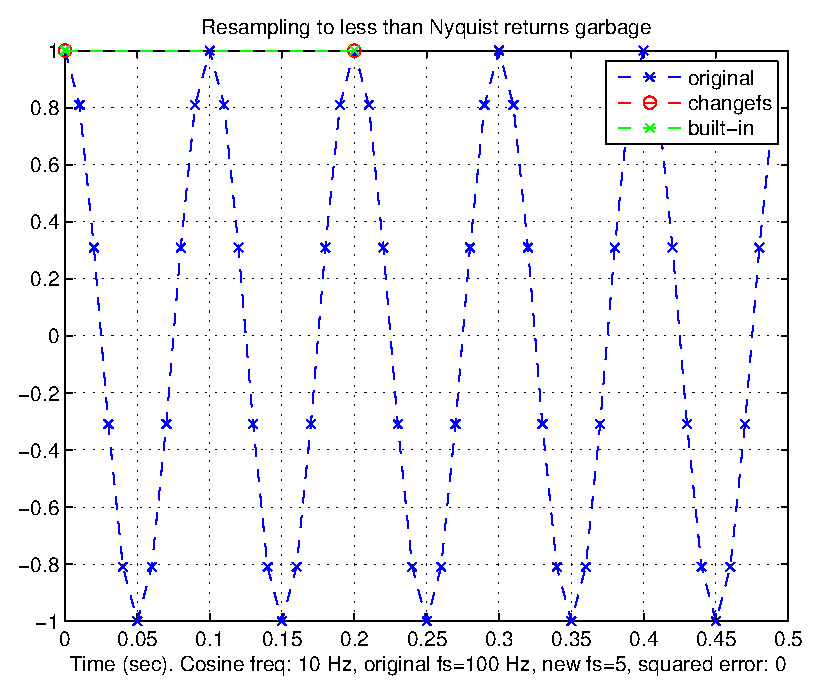
\includegraphics[width=0.35\paperwidth]{test14.eps}
  \caption{\protect{Δειγματοληψία σε συχνότητα μικρότερη της Nyquist}}
  \end{subfigure}
  %~ \hfill
\end{figure}

\par Παρατηρούμε πως τα σημεία των καμπυλών built-in και changefs ταυτίζονται, 
άρα η υλοποίησή μας είναι σωστή.
\end{minipage}
